\section{Fluxo de avaliação de vida à fadiga em dutos em vão livre}\label{chap:workflow}


Baseado nos estudos e \textit{oficinas} realizados para o desenvolvimento deste trabalho. Pôde-se estabelecer que a análise de vida a fadiga em dutos em vão livre compreende o fluxograma apresentado na \autoref{fig:fluxograma}.

\begin{figure}[!ht]
    \centering
    \caption{Fluxo de avaliação de vida à fadiga em dutos em vão livre.}\label{fig:fluxograma}
    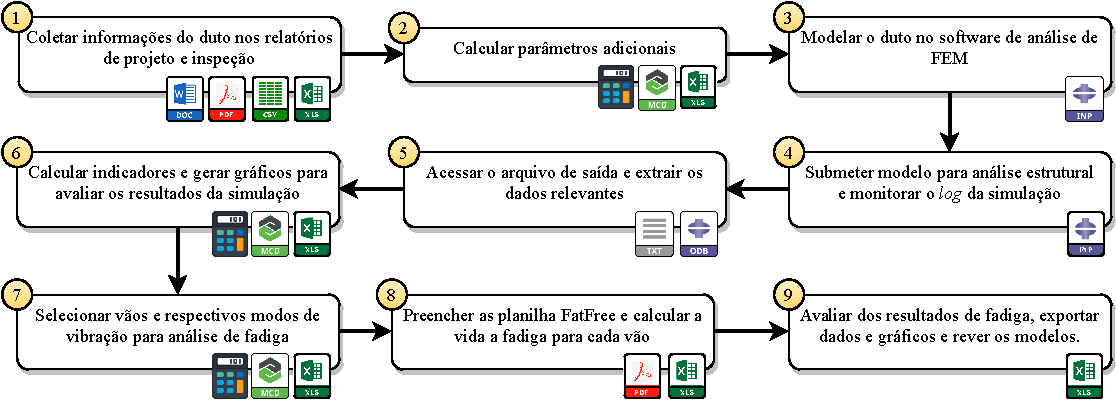
\includegraphics[width=\textwidth]{imagens/fluxograma.pdf}
    \fonte{Autor (2020)}
\end{figure}

A seguir, uma breve descrição de cada item:

\begin{enumerate}[label=(\arabic*)]
    \item Nesta etapa, o profissional reúne as informações básicas para construção dos modelos e outros dados usados em cálculos posteriores. Citadamente, temos aqui: os as cotas do perfil do duto e batimetria obtidas na inspeção, geometria e composição das camadas que compõem sessão do duto, parâmetros do solo, constantes físicas e coeficientes de segurança, posição e tipos de suportes ao longo do duto. Essa tarefa envole olhar uma série de documentos (\texttt{.doc}, \texttt{.pdf}, etc) em busca desses valores, dispostos de forma não estruturada. Quando estruturados, em forma de arquivos CSV ou planilhas, por exemplo, é necessário ainda manipular esses dados a fim de extrair somente a informação necessária ou convertê-las no formato apropriado. Um exemplo disso são os dados de batimetria, que precisam convertidos nas coordenadas dos nós de uma malha de elementos finitos.
    \item 
\end{enumerate}{}